\documentclass{article}
%encoding
%--------------------------------------
\usepackage[T1]{fontenc}
\usepackage[utf8]{inputenc}
%--------------------------------------
 
%Portuguese-specific commands
%--------------------------------------
\usepackage[portuguese]{babel}
%--------------------------------------
 
%Hyphenation rules
%--------------------------------------
\usepackage{hyphenat}
\hyphenation{mate-mática recu-perar}
%--------------------------------------


\title{Trabalho Prático 1: Otimização não Linear}
\author{Aluna: Ana Luiza Almeida Soares
\\Professor: Rodrigo César Pedrosa Silva}

\date{\today}

\usepackage{natbib}
\usepackage{graphicx}
\usepackage{amsmath}
\usepackage{makecell}
\usepackage{subfigure}

\begin{document}

\maketitle

\section{Introdução}

Este trabalho tem como objetivo realizar uma análise comparativa do desempenho de três métodos de otimização apresentados na disciplina de Otimização não Linear. Os métodos em questão são:

\begin{itemize}
  \item Gradiente Descendente com passo adaptativo padrão;
  \item Gradiente Descendente com passo adaptativo pela seção áurea;
  \item Gradiente Descendente com passo adaptativo pela regra de Armijo. 
\end{itemize}

A implementação das funções foi desenvolvida com base no código fornecido pelo professor Rodrigo César Pedrosa Silva, disponível no repositório da disciplina\footnote{https://github.com/AnaLuiza241/trabalho1\_otimizacao\_nao\_linear}.

As funções de teste que serão otimizadas são as seguintes:

\begin{equation}
  f_1(x_0, x_1) = x_0 - x_1 + 2x_0^2 + 2x_0x_1 + x_1^2;
\end{equation}
\begin{equation}
  f_2(x_0, x_1) = 10x_0^2 + 2x_1^2;
\end{equation}
\begin{equation}
  f_3(x_0, x_1) = 2x_0^2 + x_1^2 + 2x_0x_1.
\end{equation}

\section{Análise das Iterações da Função}

Um aspecto crucial para avaliar as funções de otimização é a quantidade de iterações necessárias para atingir o mínimo. As funções implementadas utilizam uma tolerância que determina quando o algoritmo deve parar. Ou seja, ao atingir essa tolerância, a função retorna o resultado encontrado. Inicialmente, optou-se por criar um histograma que compara as funções para cada método, considerando a tolerância padrão de $0.000001$. A Figura \ref{fig:hist_funcoes} apresenta esse histograma.

Observa-se que, para as funções 1 e 3, os três métodos obtiveram resultados semelhantes, com mais de 200 iterações. Embora esse resultado tenha surpreendido a autora, o número de iterações ainda é considerado baixo. Por outro lado, a função 2 teve um comportamento distinto. Os métodos que utilizam a regra de Armijo e a seção áurea destacaram-se, atingindo cerca de 50 iterações, com a regra de Armijo apresentando um número ligeiramente inferior ao da seção áurea. Por outro lado, o método adaptativo padrão teve o desempenho mais fraco, exigindo mais de 75 iterações.


\begin{figure}[h]
  \centering
  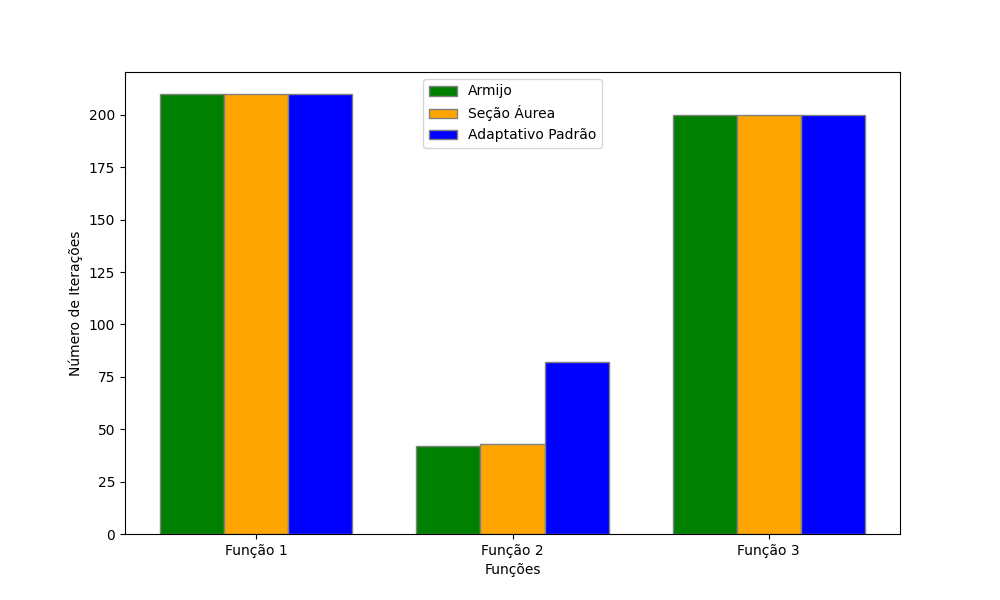
\includegraphics[width=0.9\textwidth]{histogram.png}
  \caption{Histograma de funções por número de iterações para a tolerância de $0.000001$}
  \label{fig:hist_funcoes}
\end{figure}

Para analisar o desempenho de cada método em relação às funções, assim como o comportamento ao alterar algum hiperparâmetro, foram escolhidas quatro tolerâncias diferentes. Gráficos foram então criados para cada função.

Nas Figuras \ref{fig:graf_funcao1} e \ref{fig:graf_funcao3}, observamos que para as funções 1 e 3, os três métodos (Gradiente Descendente com passo adaptativo padrão, Gradiente Descendente com passo adaptativo pela seção áurea, e Gradiente Descendente com passo adaptativo pela regra de Armijo) apresentam um comportamento bastante semelhante em relação ao número de iterações para todas as tolerâncias consideradas. Esse padrão já havia sido notado no histograma apresentado na Figura \ref{fig:hist_funcoes}, sugerindo que talvez haja uma característica específica das funções ou, alternativamente, um possível erro no desenvolvimento dos métodos. Uma análise mais aprofundada é necessária para entender melhor esse comportamento consistente.


Analisando a Figura \ref{fig:graf_funcao2}, é evidente que o método adaptativo padrão se destaca negativamente, apresentando um maior número de iterações em comparação com os métodos da regra de Armijo e seção áurea para todas as tolerâncias avaliadas. Interessantemente, os métodos da regra de Armijo e seção áurea mostram um desempenho bastante similar, com sobreposição de linhas em algumas tolerâncias. Contudo, é crucial notar que o método da regra de Armijo possui um desempenho mais levemente mais eficiente eficiente, com um menor número de iterações, especialmente nas tolerâncias mais baixas.

\begin{figure}[h]
  \centering
  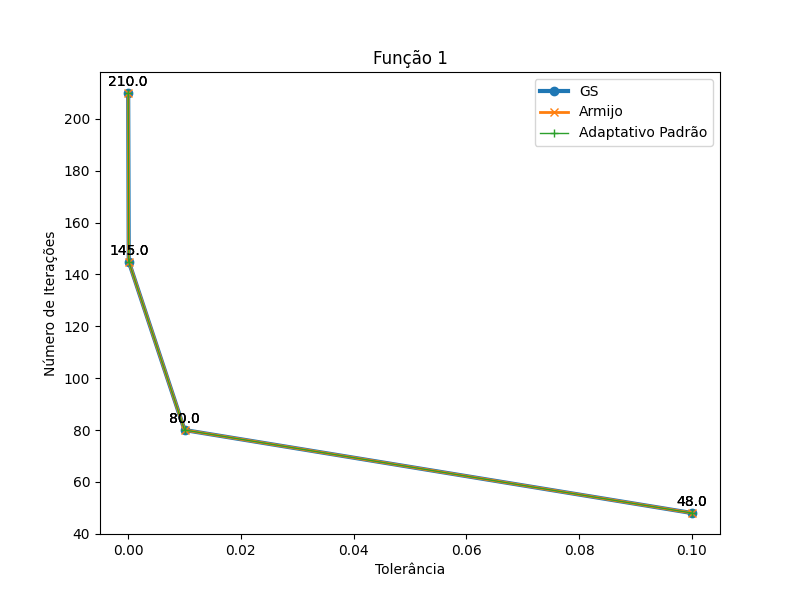
\includegraphics[width=0.9\textwidth]{funcao_1_otimizacao.png}
  \caption{Gráfico de tolerância em função do número de iterações para a Função 1.}
  \label{fig:graf_funcao1}
\end{figure}

\begin{figure}[h]
  \centering
  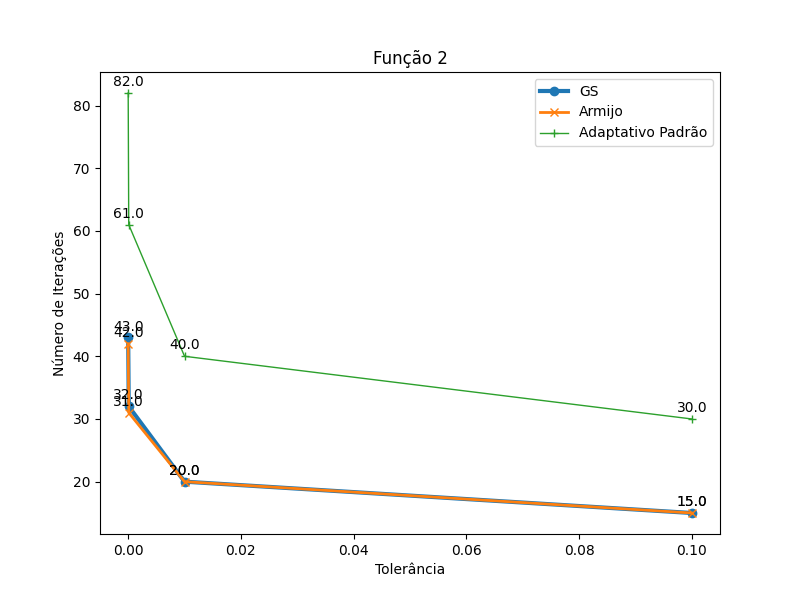
\includegraphics[width=0.9\textwidth]{funcao_2_otimizacao.png}
  \caption{Gráfico de tolerância em função do número de iterações para a Função 2.}
  \label{fig:graf_funcao2}
\end{figure}

\begin{figure}[h]
  \centering
  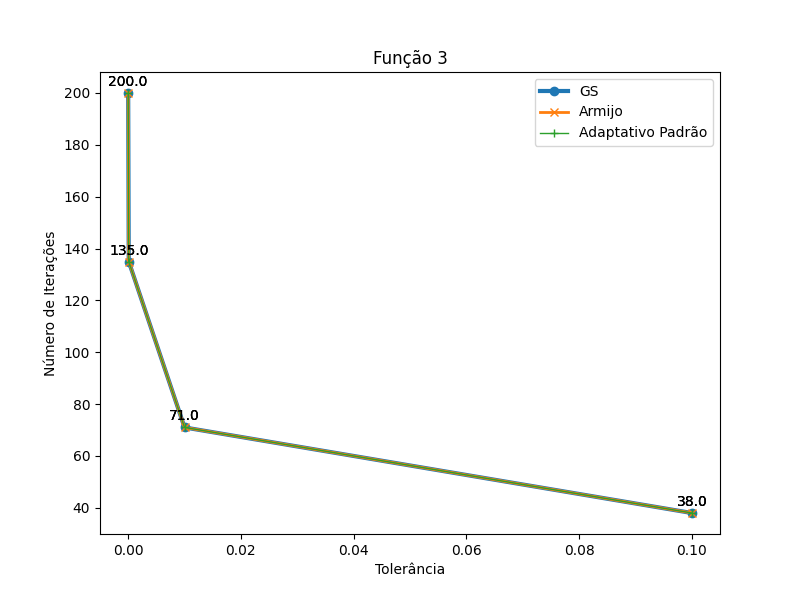
\includegraphics[width=0.9\textwidth]{funcao_3_otimizacao.png}
  \caption{Gráfico de tolerância em função do número de iterações para a Função 3.}
  \label{fig:graf_funcao3}
\end{figure}


\bibliographystyle{plain}
\bibliography{references}
\end{document}
